\documentclass[tikz,border=2pt]{standalone}
\usetikzlibrary{arrows.meta,positioning,calc,shapes.geometric}
\usepackage{fontspec}
\setmainfont{TeX Gyre Termes}
\setsansfont{Roboto}
\begin{document}
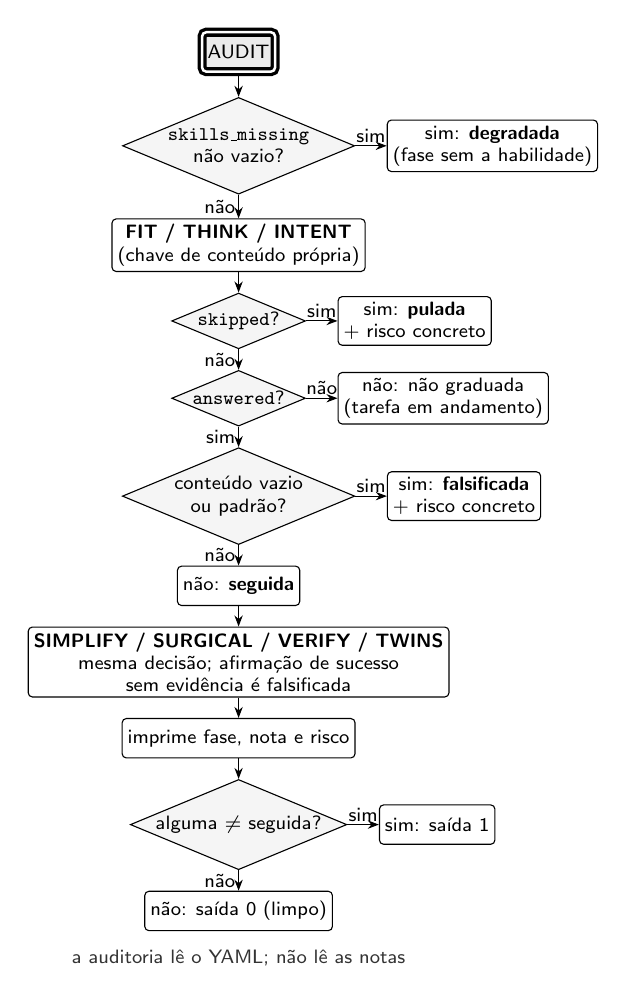
\begin{tikzpicture}[
  font=\sffamily\scriptsize, >={Stealth[length=4pt]},
  proc/.style={draw, thin, rounded corners=1.5pt, align=center, fill=white, minimum height=0.5cm, inner sep=2pt},
  exec/.style={proc, very thick, double distance=0.9pt, fill=black!8},
  dec/.style={draw, thin, diamond, aspect=2.4, align=center, fill=black!4, inner sep=0.5pt, font=\sffamily\scriptsize},
  nota/.style={font=\sffamily\scriptsize, align=center, text=black!80},
  lbl/.style={font=\sffamily\scriptsize, inner sep=1pt}
]
\node[exec] (a) {AUDIT};
\node[dec, below=0.3cm of a] (pf) {\texttt{skills\_missing}\\ não vazio?};
\node[proc, right=0.4cm of pf] (pfd) {sim: \textbf{degradada}\\ (fase sem a habilidade)};
\node[proc, below=0.3cm of pf] (f1) {\textbf{FIT / THINK / INTENT}\\
  (chave de conteúdo própria)};
\node[dec, below=0.26cm of f1] (sk) {\texttt{skipped}?};
\node[proc, right=0.4cm of sk] (skd) {sim: \textbf{pulada}\\ + risco concreto};
\node[dec, below=0.26cm of sk] (an) {\texttt{answered}?};
\node[proc, right=0.4cm of an] (ang) {não: não graduada\\ (tarefa em andamento)};
\node[dec, below=0.26cm of an] (emp) {conteúdo vazio\\ ou padrão?};
\node[proc, right=0.4cm of emp] (empd) {sim: \textbf{falsificada}\\ + risco concreto};
\node[proc, below=0.26cm of emp] (fo) {não: \textbf{seguida}};
\node[proc, below=0.26cm of fo] (resto) {\textbf{SIMPLIFY / SURGICAL / VERIFY / TWINS}\\
  mesma decisão; afirmação de sucesso\\
  sem evidência é falsificada};
\node[proc, below=0.26cm of resto] (out) {imprime fase, nota e risco};
\node[dec, below=0.26cm of out] (ex) {alguma $\ne$ seguida?};
\node[proc, right=0.4cm of ex] (ex1) {sim: saída 1};
\node[proc, below=0.26cm of ex] (ex0) {não: saída 0 (limpo)};
\draw[->] (a) -- (pf);
\draw[->] (pf) -- node[lbl,above]{sim} (pfd);
\draw[->] (pf) -- node[lbl,left]{não} (f1);
\draw[->] (f1) -- (sk);
\draw[->] (sk) -- node[lbl,above]{sim} (skd);
\draw[->] (sk) -- node[lbl,left]{não} (an);
\draw[->] (an) -- node[lbl,above]{não} (ang);
\draw[->] (an) -- node[lbl,left]{sim} (emp);
\draw[->] (emp) -- node[lbl,above]{sim} (empd);
\draw[->] (emp) -- node[lbl,left]{não} (fo);
\draw[->] (fo) -- (resto);
\draw[->] (resto) -- (out);
\draw[->] (out) -- (ex);
\draw[->] (ex) -- node[lbl,above]{sim} (ex1);
\draw[->] (ex) -- node[lbl,left]{não} (ex0);
\node[nota, below=0.12cm of ex0] {a auditoria lê o YAML; não lê as notas};
\end{tikzpicture}
\end{document}
